%priprava posamezne ure
%tukaj zaporedoma napisemo{st. zaporedne ure}{datum}{naslov}{poglavje}{oblika dela}{pripomocki}
\begin{priprava}{}{}{Integral}{Nedoločeni integral}{frontalna}{tabla}

Grafična motivacija: Na enem primeru narišemo graf $ f $ in nato graf njenega odvoda, npr. $ x^3 - x $ in $ 3x^2 - 1 $ (ponovimo pomen odvoda). Potem pa naredimo obratno. Recimo, da imamo $ f(x) = 1 - x $ in želimo narisati graf funkcije, katere odvod je $ f $ in ki gre skozi $ (0, 0) $ (s tangentami ...).

\begin{figure}[h]
    \centering
    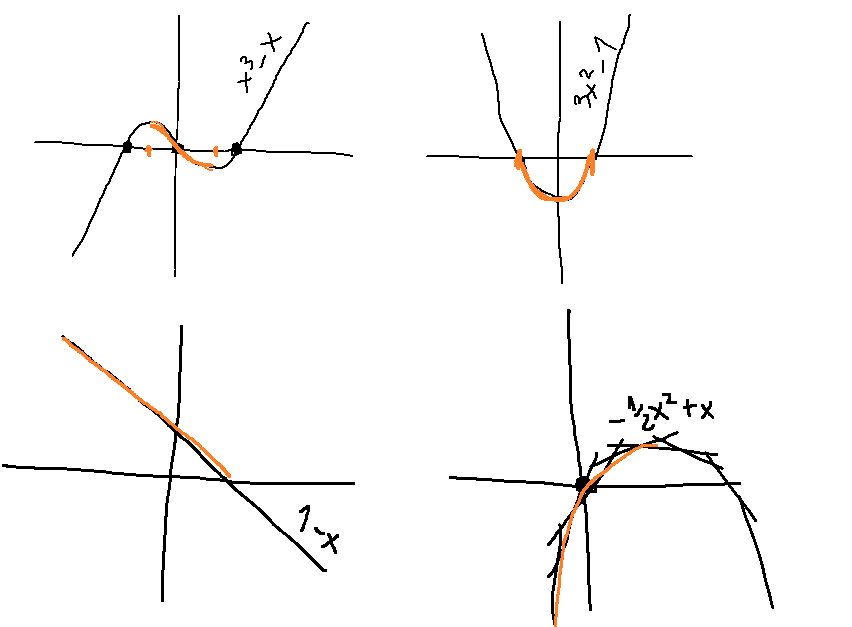
\includegraphics[width=0.6\textwidth]{slike/graf_odvod_integral.png}
\end{figure}

Računska motivacija: začnemo s tabelo, kjer vrstice sproti pišeš. Po treh primerih pa se vaja obrne. \vaje{Katero funkcijo smo odvajali, da smo dobili $ f(x) = 4x - 3 $?} 

\begin{center}
\begin{tabular}{ |c|c| } 
     $ F(x) $ & $ F'(x) = f(x) $ \\
     \hline \hline $ 3x^2 - 5 $ & \\
     \hline $ 6x $ & \\
     \hline $ 2 \cos{\frac{x}{2}} $ & \\
     \hline & $ 4x - 3 $ \\
     \hline & $ \frac{1}{2} \cos x $ \\
     \hline & $ e^{-x} $ \\
     \hline
\end{tabular}
\end{center}

\didopomba{Zadnje 3 primere naj sami poskušajo ugotoviti, ker znajo odvajati $ \rightarrow 2x^2 - 3x $. Rešijo vse tri primere. Potem pa vsakemu prišteješ še neko naključno konstanto, kaj pa ta funkcija, ali je tudi ta vredu? Naj pogruntajo, da lahko dobljeni funkciji prištejejo katerokoli konstanto in se njen odvod s tem ne spremeni.}

Problem: Iščemo $ F(x) $, za katero velja $ F'(x) = f(x) $. Ker je $ c' = 0 $, lahko $ F(x) $ določimo do konstante natančno: $ F(x) + c $. Določanju take funkcije pravimo \textbf{integriranje}.

\newpage


\begin{figure}[h]
    \centering
    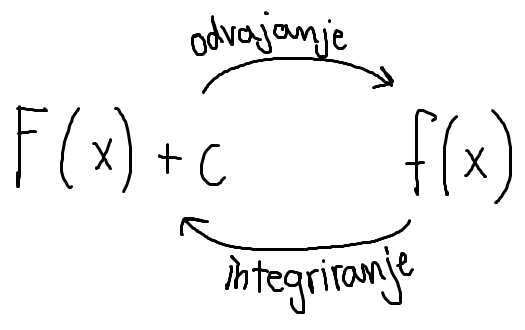
\includegraphics[width=0.3\textwidth]{slike/povezava_F(x)_f(x).png}
\end{figure}


\textbf{Nedoločen integral funkcije $ f(x) $ je funkcija, katere odvod je enak $ f(x) $.} Označimo jo z $ \int f(x) dx $.

$$
    \int f(x) dx = F(x) + c \Longleftrightarrow (F(x) + c)' = F'(x) = f(x)
$$

\didopomba{Napišemo zraven ob strani na enak način še en primer iz tabele:}

$$
    \int (4x - 3) dx = 2x^2 - 3x + c \Longleftrightarrow (2x^2 - 3x + c)' = 4x - 3
$$

\textcolor{rdeca}{Razlaga oznak $ \int $ in $ dx $:} Izhaja iz oznake pri določenem integralu, ki ga bomo spoznali kasneje. Zdaj se učimo nedoločen integral, s katerim bomo lahko računali določene. Oznaka $ dx $ tudi pove, po kateri spremenljivki integriramo (npr. če je v integralu več črk, vse razen $ x $ obravnavamo kot konstante). Ni treba preveč se trudit, pač ga bomo potrebovali kasneje (pri uvedbi nove spremenljivke in določenem integralu).

\naslov{Tabela integralov}

\didopomba{Naj bo enake oblike kot pri odvodih (če je bila tam po alinejah, naj bo tudi tu itd.) Naj pravila sami pogruntajo.}

\begin{itemize}
    \item $ \int k dx = kx + c $
    \item $ \int x^n dx = \frac{x^{n+1}}{n + 1} + c; n \ne -1 $
    \item $ \int \frac{1}{x} dx = \ln |x| + c $ \didopomba{od kje pride absolutna (TO POGLEJTE ŽE PRI ODVODIH!!!)? funkcijo $ \ln |x| $ se spozna (funkcijo $ \ln x $ se samo preslika še na desno stran), in jo lahko odvajamo na vsaki strani osi, v obeh primerih dobiš odvod enak $ 1/x $ ne glede na predznak $ x $.}
    \item $ \int e^x dx = e^x + c $
    \item $ \int a^x dx = \frac{a^x}{\ln a} + c $
    \item $ \int \sin x dx = - \cos x + c $
    \item $ \int \cos x dx = \sin x + c $
    \item $ \int \frac{1}{\cos^2 x} dx = \tan x + c $
    \item $ \int \frac{1}{\sin^2 x} dx = - \cot x + c $
    \item $ \int \frac{1}{\sqrt{1-x^2}} dx = \arcsin x + c $
    \item $ \int \frac{-1}{\sqrt{1-x^2}} dx = \arccos x + c $
    \item $ \int \frac{1}{x^2 + 1} dx = \arctan x + c $

\end{itemize}


\newpage

% Lastnosti

\naslov{Pravila}
\didopomba{sledijo iz odvajanja}
\begin{itemize}
    \item $ \int(f(x) \pm g(x)) dx = \int f(x) dx \pm \int g(x) dx $
    \item $ \int c \cdot f(x) dx = c \int f(x) dx $ 
    \item za produkt in količnik (kot pri odvodu) to ne gre! \\
            \didopomba{Primer: $ \int 2x dx \ne \int 2 dx \cdot \int x dx $, $ \int \frac{x}{2} dx \ne \frac{\int x dx}{\int 2 dx} $}
\end{itemize}


\vaje{
Vaje: 
\begin{itemize}
    \item Začnemo postopoma, z osnovnimi integrali, s + in -, nato kakšno racionalno, kotne funkcije, pač golo računanje, MENJUJEMO ČRKE (ne le $ x $) \dots
    \item Primer iz uvodne motivacije: Poišči predpis za funkcijo, ki gre skozi $ A(0,0) $ in je njen odvod enak $ g'(x) = 1 - x $. \didopomba{spet najprej geometrijsko, potem pa se še računsko prepričamo}
\end{itemize}
}

\naslov{Uvedba nove spremenljivke}

\vaje{Izračunaj integral $ \int (3x - 4)^6 dx $.}

\didopomba{Ni treba pisati postopka. Lahko bi izračunali šesto potenco izraza, vendar obstaja lažja pot. Označimo izraz $ 3x - 4 $ s spremenljivko, npr. s $ t $ ($ t $ je sedaj funkcija $ x $) in to vstavimo v integral}: $ \int t^6 dx $ \didopomba{V integralu je $ t $, ampak mi integriramo po $ x $, torej bo treba nekaj popravit \ldots}

$ t = 3x - 4 $ \didopomba{sedaj uporabimo znanje od diferencialih}\\
$ dt = t' dx = 3 dx \rightarrow dx = \frac{dt}{3} $ \\
$ \int (3x - 4)^6 dx = \int t^6 \frac{dt}{3} = \int \frac{t^6}{3} dt = \frac{t^7}{3 \cdot 7} + c = \frac{(3x - 4)^7}{21} + c $

\didopomba{Še en način: namesto, da izraz označimo s črko $ t $, ga že zapišemo z diferenciali namest $ dx $ (v bistvu gre za isto stvar, le da ne uporabimo nove oznake)}

$ \int (3x - 4)^6 dx = \int (3x - 4)^6 \frac{d(3x - 4)}{3} = \frac{1}{3} \int \square^6 d \square = \frac{1}{3} \frac{\square^7}{7} + c = \frac{(3x - 4)^7}{21} + c $

\vaje{
Vaje: 
\begin{itemize}
    \item Veliko izbire za golo računanje \dots
    \item $ \int \frac{3x^2}{x^3 + 2} dx \rightarrow \int \frac{f'(x)}{f(x)} dx = \ln |f(x)| + c $
    \item $ \int \frac{dx}{x^2 + 4} \rightarrow \int \frac{dx}{x^2 + a^2} = \frac{1}{a} \arctan \frac{x}{a} + c $
    \item $ \int \frac{x^2 + 2x - 1}{x^2 - 1} dx $: če je stopnja števca $ \geq $ stopnja imenovalca, se deli in posebej integrira.
    \item $ \int \frac{2}{1 - x^2} dx $: če je stopnja števca $ < $ stopnja imenovalca in se ne da zlahka integrirat, se izraz razstavi s pomočjo parcialnih ulomkov: \\
    $ \frac{2}{1 - x^2} = \frac{A}{1 - x} + \frac{B}{1 + x} $ \ldots
    \item $ \int \cos x \sin{2x} dx $ (uporaba dvojnih kotov)
\end{itemize}
}

\newpage


\naslov{Per partes (integriranje po delih)}

\didopomba{Uvodni primer za motivacijo, ker ga ne znamo z novo spremenljivko rešit ...}

\vaje{$ \int x e^x dx = $ ?}

Radi bi integral preoblikovali v obliko, ki bi jo znali rešiti:

\begin{figure}[h]
    \centering
    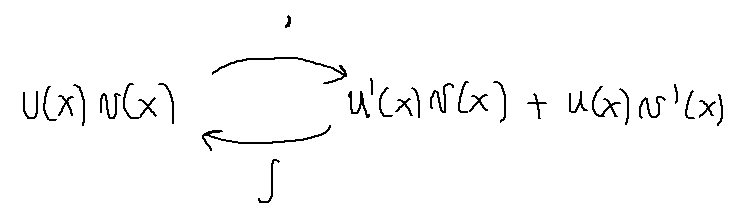
\includegraphics[width=0.6\textwidth]{slike/perpartes1.png}
\end{figure}

Torej $ u(x) \cdot v(x) = \int u'(x)v(x) dx + \int u(x)v'(x)dx $

\didopomba{Zaradi boljše preglednosti spustimo argument $ (x) $ ter preuredimo z diferenciali v obliko:}

$ u \cdot v = \int u' v dx + \int u v'dx = \int v du + \int u dv $ \didopomba{kjer sta $ u'(x)dx = du, v'(x)dx = dv $}

\text{Običajno zapišemo v obliki } \textcolor{rdeca}{$ \int u dv = u \cdot v - \int v du $}

\didopomba{Večkrat je integral na desni enostavnejši od levega. Za $ u $ običajno daš tisti del, ki se z odvajanjem poenostavi. Na koncu rezultat odvajamo, da preverimo, ali smo prav.}

\begin{tabular}{l l}
    $ u = x $ & $ dv = e^xdx $ \\
    $ du = dx $ & $ v = e^x $
\end{tabular}

\didopomba{pri integriranju $ dv $ ne pišemo $ c $-ja, ker bo konstanta prišla ven tudi pri novonastalem integralu}

$ \int x e^x dx = x \cdot e^x - \int e^x dx = e^x (x - 1) + c $

\vaje{
Vaje: 
\begin{itemize}
    \item $ \int x \sin x dx $
    \item $ \int \ln x dx $
    \item $ \int x^3 \ln x dx $
    \item $ \int e^x sin x dx $ Dvakratni per partes! \didopomba{$ u = e^x $}
\end{itemize}
}

\vaje{
Še kakšne posebne vaje:
\begin{itemize}
    \item Dan odvod funkcije in točka, skozi katero gre (poišči to funkcijo)
    \item $ \int cos x sin 3x dx $ zahteva uporabo $ sin x cos y = \frac{1}{2} (sin(x-y) + sin (x+y)) $
\end{itemize}
}

    
\end{priprava}